\subsection{G 上的中心函数与 T 上的函数}

记 \(\mathcal{C}(\mathrm{G})\) 为 G 上连续复值函数所成的空间，记 \(\mathcal{C}^{\infty}(\mathrm{G})\) 为无穷次可微函数所成的子空间。于是有包含链

\[
\Theta (\mathrm{G}) \subset \mathscr {C} ^ {\infty} (\mathrm{G}) \subset \mathscr {C} (\mathrm{G}) \subset \mathrm{L} ^ {2} (\mathrm{G}).
\]

分别记 \(Z\Theta(G)\)、\(Z\mathcal{C}^{\infty}(G)\)、\(Z\mathcal{C}(G)\)、\(ZL^{2}(G)\) 为这些空间中由中心函数组成的子空间。类似地引入空间 \(\Theta(T)\)、\(\mathcal{C}^{\infty}(T)\)、\(\mathcal{C}(T)\)、\(L^{2}(T)\)；对于此列表中的任意空间 E，记 \(E^{W}\)（相应地，\(E^{-W}\)）为由 Weyl 群 W 的作用下不变（相应地，反不变）元素组成的子空间。有交换图

\[
\begin{array}{c c c} \mathsf {Z C} (\mathsf {G}) & \stackrel {{a _ {c}}} {{\longrightarrow}} & \mathcal {C} (\mathsf {T}) ^ {\mathsf {W}} \\ \uparrow & & \uparrow \\ \mathsf {Z C} ^ {\infty} (\mathsf {G}) & \stackrel {{a _ {\infty}}} {{\longrightarrow}} & \mathcal {C} ^ {\infty} (\mathsf {T}) ^ {\mathsf {W}} \\ \uparrow & & \uparrow \\ \mathsf {Z} \Theta (\mathsf {G}) & \stackrel {{a _ {\Theta}}} {{\longrightarrow}} & \Theta (\mathsf {T}) ^ {\mathsf {W}} \end{array}
\]

其中竖直箭头表示典则嵌入，映射 \(a_{c}, a_{\infty}, a_{\Theta}\) 由从 \(\mathcal{C}(G)\) 到 \(\mathcal{C}(T)\) 的限制映射诱导。

映射 \(a_c, a_\infty, a_\Theta\) 都是双射（§2, no. 5, Cor. 1 of Prop. 5, §8, no. 3, Cor. of Prop. 5, and §7, no. 3, Cor. of Prop. 2）。

现在假设正根的半和 \(\rho\) 属于 X(T)，并考虑映射 b，它将 T 上的每个连续函数 \(\varphi\) 赋予 \(\varphi\cdot\mathrm{J}(\rho)\)。有交换图

\pandocbounded{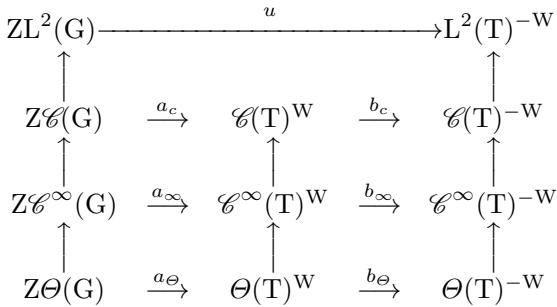
\includegraphics[keepaspectratio]{images/part003_8b0b3ceb.jpg}}

其中竖直箭头是典则包含映射，映射 \(b_{c}, b_{\infty}, b_{\Theta}\) 由 b 诱导，而 u 通过连续性延拓 \(b_{c} \circ a_{c}\)（§7, no. 4, Cor. 3 of Th. 2）。映射 u 和 \(b_{\Theta}\) 是双射（loc. cit.）；\(b_{\infty}\) 也是双射（Exerc. 5）；另一方面，\(b_{c}\) 一般不是满射（Exerc. 6）。

